
\section{Experimento - Determinação da distância da bola ao robô}

Os cálculos das distâncias da bola e do robô até outros robôs, foram determinados de forma experimental, tabelando a distância em centímetros e a área dos objetos em pixels, encontrando uma função que representasse essa relação, considerando a resolução da captura. As funções experimentais obtidas, por meio de regressão, estão nos algoritmos propostos.


O principal objetivo da média móvel simples é fornecer o valor médio do raio da bola e sua posição em pixels dentro de um determinado período, no caso, os últimos 10 quadros da captura de video. Assim, para cada valor incluído no cálculo da média, o valor mais antigo é excluído. Na média móvel simples (SMA), cada dado utilizado no cálculo da média terá o mesmo peso. 

\begin{equation} 
	MRB = \frac {[R(q) + R(q-1) + R(q-2) + … + R(q-9)]}  {10}
\end{equation}\\

MRB é a média móvel do raio da bola e R é o raio da bola ambos em pixels, já "q" se refere ao indice do quadro atual da captura da camera. 

Tabelando os raios médios da bola e sua distância real em centímetros, é possível por meio de regressão estimar uma função que representa os dados. 30 pontos foram levantados com varições A bola foi posicionada à 50 centimetros do pé do robô, para cada incremento de 5 centimetros o raio médio da bola foi coletado, 

\begin{equation} 
	%D_{bola} = 3,7.10^{-7} * MRB^4 -7.9e^{-5} * MRB^3 +6.2e^{-3} * MRB^2 -2.2e^{-1} * MRB + 3.7 
	%D_{bola} = 331.59-53.3*log(MRB-50);
	D_{bola} = \frac {9143} {MRB}
\end{equation}\\

Essa função foi extraída para a resolução de 1920x1080 e bola de tamanho fixo conhecido de 13 centímetros, onde \(D_{\text{Bola}}\) é a distância da bola ao robô em centimetros, e MRB é a média móvel do raio da bola em pixels.

\begin{figure}[!t1]
\centering
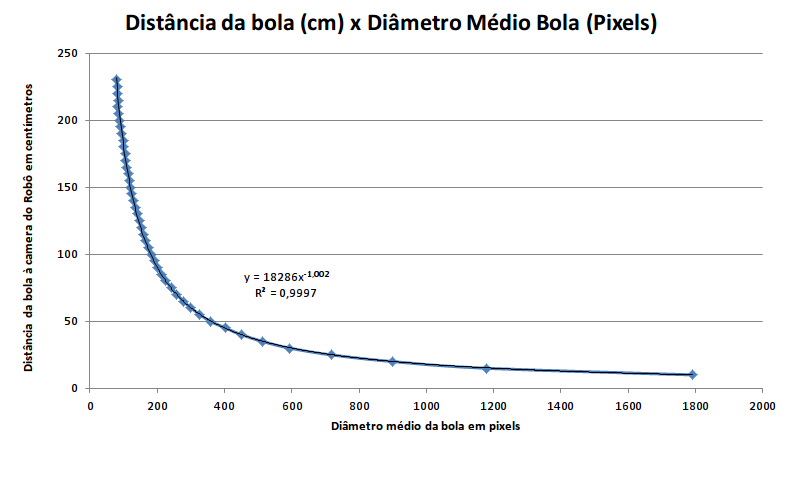
\includegraphics[width=10cm]{Imagens/Dist.png}
\DeclareGraphicsExtensions.
\caption{Função relacionando pixels com distância de uma bola de tamanho conhecido.}
\label{Fig:DistBall}
\end{figure}

É claro que, haverá um erro de medição nessas fórmulas, já que foram calculadas sem oclusão e com o objeto inteiro no campo de visão, nesse caso, o erro será proporcional à oclusão.


\section{Experimento - Determinação da distância do robô a outros robôs}

Para determinar as distâncias até os robôs adversários, ou até os companheiros de equipe é necessário que se possua todas as dimensões dos robôs da liga. Analisando os TDP's Artigos de descrição dos times de todos os robôs da liga KidSize, foram extraídos as alturas dos mesmos.
A tabela criada possui uma coluna referente ao número do time e uma ou mais colunas referente à altura do robôs de cada time, já que um time pode ter mais de um tipo de robô. 

Antes de se iniciar uma partida, o juiz procura os líderes de cada time para definição de suas respectivas cores. Duas cores são possíveis, o time vermelho tem uma coloração magenta e o time azul tem a cor ciano. Feita a escolha, os times devem revestir seus robôs com as cores definidas. A área mínima desses marcadores é 5x5 centímetros nos braços, pernas e tronco.

A abordagem experimental será abordada para esse caso, 

A detecção foi feita usando o descritor HAAR conforme parametros usados no capitulo ~\ref{HAAR-Boosting}

Somente dentro da janela de detecção do robô é feita uma segmentação da cor previamente escolhida no sistema HSV. Os valores foram discretizados em 20 valores para a matiz, 17 para a saturação e 17 para a intensidade.
Visto que para a resolução de 1920x1080 pixels a relação dis

Assim, se faz necessário encontrar uma fórmula que relacione a resolução da tela, o tamanho em pixels e o tamanho real do robô com a sua distância.

\pagebreak
